\begin{figure}[t]
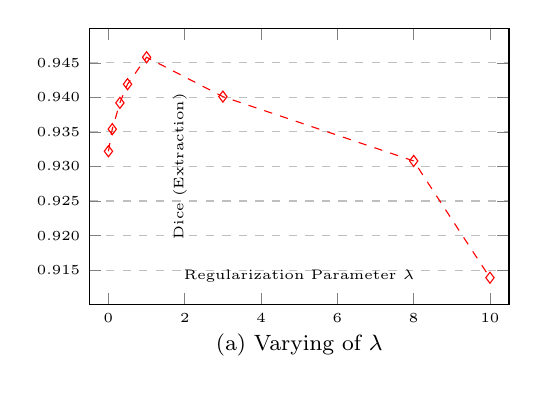
\begin{tikzpicture}
\begin{axis}[
    % inner sep=0,
    title = {(a) Varying of $\lambda$},
    outer sep=0,
    width=0.57\columnwidth,
    height=0.42\columnwidth,
    xlabel={Regularization Parameter $\lambda$},
x label style={at={(axis description cs:0.5,0.16)},anchor=north},
y label style={at={(axis description cs:0.254,.5)},anchor=south},
    % xlabel near ticks,
    % ylabel near ticks,
    ylabel={Dice (Extraction)},
    xmin=-0.5, xmax=10.5,
    ymin=0.910, ymax=0.950,
    xtick={0,2,4,6,8,10},
    ytick={0.915, 0.920, 0.925, 0.930, 0.935,0.940, 0.945},
    yticklabels={0.915, 0.920, 0.925, 0.930, 0.935,0.940, 0.945},
    ymajorgrids=true,
    grid style=dashed,
    tick label style={font=\tiny},
    label style={font=\tiny},
    title style={font=\footnotesize,align=center, yshift=-0.37\columnwidth},
]

\addplot[
    dashed,
    color=red,
    mark=diamond,
    mark options=solid,
    ]
    coordinates {
    (0,0.9322)(0.1,0.9354)(0.3,0.9392)(0.5,0.9419)(1.0,0.9458)(3.0,0.9401)(8.0,0.9308)(10.0,0.9139)
    };

\end{axis}
\end{tikzpicture}
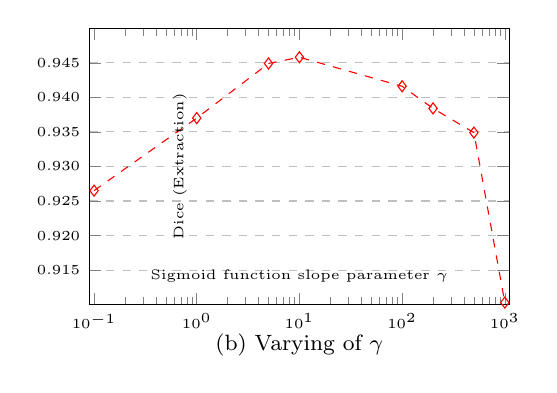
\begin{tikzpicture}
\begin{semilogxaxis}[
    %log ticks with fixed point,
    % extra x tick style={
    % log identify minor tick positions=true,
    % },
    % inner sep=0,
    title = {(b) Varying of $\gamma$},
    outer sep=0,
    width=0.57\columnwidth,
    height=0.42\columnwidth,
    xlabel={Sigmoid function slope parameter $\gamma$},
x label style={at={(axis description cs:0.5,0.16)},anchor=north},
y label style={at={(axis description cs:0.254,.5)},anchor=south},
    ylabel={Dice (Extraction)},
    xmin=0.09, xmax=1100,
    ymin=0.910, ymax=0.950,
    xtick={0.1, 1, 10, 100, 1000},
    ytick={0.915, 0.920, 0.925, 0.930, 0.935,0.940, 0.945},
    yticklabels={0.915, 0.920, 0.925, 0.930, 0.935,0.940, 0.945},
    ymajorgrids=true,
    grid style=dashed,
    tick label style={font=\tiny},
    label style={font=\tiny},
    title style={font=\footnotesize,align=center, yshift=-0.37\columnwidth},
]

\addplot[
    dashed,
    color=red,
    mark=diamond,
    mark options=solid,
    ]
    coordinates {
    (0.1,0.9265)(1,0.9370)(5,0.9449)(10,0.9458)(100,0.9416)(200,0.9384)(500,0.9349)(1000,0.9103)
    };

\end{semilogxaxis}
\end{tikzpicture}
    \vspace{-10pt}
     \caption{Effect of varying the mask smoothing regularization parameter $\lambda$ and sigmoid function slope parameter $\gamma$.}
    \label{fig:lambda}
    \vspace{-10pt}
\end{figure}

